\documentclass{article}
\usepackage{graphicx} % Required for inserting images
\usepackage{amsmath,amssymb,amsfonts}
\usepackage{algorithmic}
\usepackage{textcomp}
\usepackage{float}
\usepackage{etoolbox}
\usepackage{hyperref}
\usepackage{tikz}
\usepackage{fontawesome}
\usepackage{caption}
\usepackage{url}
\usepackage{listings}
\usepackage{pdfpages}
\usepackage[english]{babel}
\usepackage{scalerel}
\usepackage{xcolor,colortbl}
\usepackage[ruled,vlined]{algorithm2e}
\usepackage{amsmath}
\usepackage{amssymb}
\usepackage{multirow}

\title{A Voter-to-Voter Internet Voting Protocol}
\author{Stanislaw Baranski and Lev Soukhanov}
\date{May 2023}

\begin{document}

\maketitle

\section{Introduction}
Voting is one of the most popular mechanisms for collective decision-making, prevalent in all types of communities including: non-government organizations, boardrooms, housing associations, regional contests and plebiscites, domestic presidential elections, as well as all forms of global voting that take place on the internet.

The act of vote can occur in different ways including paper-based precinct voting, mail-in ballots, electronically using direct-recording electronic (DRE) voting machine, and internet voting~\cite{parkGoingBadWorse2021}.

As proposed by Vitalik Buterin\cite{buterinBlockchainVotingOverrated2021} each voting (or more broadly, each collective decision-making) method faces a trilemma allowing it to choose only two out of three properties:

\begin{itemize}
    \item \textbf{Democratic}, means that the method ensures easy and equal (egalitarian) decision input for all eligible voters;
    \item \textbf{Secure}, means that the voting is confident, fair, transparent, private, and resistant to attack vectors;
    \item \textbf{Efficient}, means that the method is easy, fast, and cheap.
\end{itemize}

In traditional political elections, security and democracy are essential factors, thus efficiency is sacrificed. Social media votings are democratic and efficient, thus security is sacrificed. An example of an efficient and secure collective decision-making mechanism is the market, where users express their preferences by purchases, increasing the lobbying power of such a company. Markets, however, are not democratic, making them a poor fit for decisions regarding public goods. 

The inefficiency of traditional voting makes them costly and thus limits their frequency usually to a single vote once every one to six years~\cite{buterinBlockchainVotingOverrated2021}.

Voting over the internet (i-voting) seems to be an ideal solution especially when online banking is so prevalent nowadays. Arguably, internet voting is the most conventional, cheapest, fastest, and safest (e.g., during the outbreak of COVID-19), and hence, a preferred method for conducting voting.

Internet voting can increase turnout and the frequency of votings, but most importantly, it can catalyze the further development of modern democracy. Enabling practical applications of direct democracy, liquid democracy, and all other sorts of voting methods like Quadratic Voting, Approval voting, Alternative vote, Score voting, and many others \cite{laslierLoserPluralityVoting2011}.

Moreover, visions of smart cities, crypto cities \cite{buterinCryptoCities2021}, Decentralised Autonomous Organisations (DAO)~\cite{wangDecentralizedAutonomousOrganizations2019}, and other forms of algorithmic governance~\cite{GovernmentAlgorithm2022} rely heavily on the existence of electronic voting, so there is a high need for such systems, as they would enable further development of modern democracy.

Undoubtedly, there is a high demand for internet voting protocol. However, except a minor cases like Switzerland and Estonia, the progress of introducing modern democracy tools is still slow comparing to e.g., online banking.

Internet voting has been researched for many years, especially in domains such as cryptography, which is an inevitable part of system security. Many of them doubt the possibility of conducting public voting over the internet \cite{parkGoingBadWorse2021, mearianWhyBlockchainbasedVoting2019, shanklandNoBlockchainIsn2018, leeBlockchainbasedElectionsWould2018, schneierBlockchainVoting2020, schneierBlockchainTrust2019}. The resistance lies—among others—in insufficient confidence in the technology and a need for trust in the authorities controlling the voting process.

The criticism against internet voting comes down to two arguments:

\begin{enumerate}
    \item No software is flawless, therefore it can not be trusted.
    \item There is too strong a trust assumption in authorities controlling the voting process.
\end{enumerate}

A recent paper from MIT researchers~\cite{parkGoingBadWorse2021} argues that any paperless voting is a bad design. High-quality software (at the 90th percentile for the software industry) contains on average one defect in every ten thousand lines of code~\cite{llaguno2017CoverityScan2017}. Some errors lead to malfunctioning, and some are "exploitable vulnerabilities", which allow an adversary to take control over the computer and install fraudulent software.

The argument is that an undetected change or error in a system's software should not cause an undetectable change in the election outcome, and since every software is flawed, there is no such guarantee.

However, recent advances in cryptography can guarantee correct program execution using zero-knowledge proofs~\cite{parnoPinocchioNearlyPractical2013}. Using such a publicly available proving system, anyone can verify the correctness of the voting process. Because the proofs of correctness are just cryptographic materials, everyone can write their implementation of a verifier program, achieving the software independence requirement stated by the authors of~\cite{parkGoingBadWorse2021}.

Even if the software can be trusted, another argument is that the hardware (voters' devices) can not be trusted. They argue that "internet voting protocols' security relies upon voters' devices being uncompromised and functioning as intended, an unrealistic assumption~\cite{parkGoingBadWorse2021}.

Although hardware (even the Trusted Hardware~\cite{sionTrustedHardware2009} like Intel® Software Guard Extensions~\cite{mckeenIntelSoftwareGuard2016}) keeps getting broken~\cite{goodinIntelSGXVulnerable2020, IntelSGXBroken2019, bulckForeshadowExtractingKeys}, there is a constant improvement in the security of the hardware. Especially, smartphones are being equipped with a secure area on their main processors called Trusted Execution Environment (TEE). For example, Apple's Secure Enclaves~\cite{SecureEnclave}, Samsung's Knox~\cite{kanonovSecureContainersAndroid2016}, HTC's Zion~\cite{exodusZION}, and ARM's TrustZone~\cite{ARMSecurityTechnology}. Generally, it is believed that cybersecurity is getting better, not worst~\cite{golombBelieveItCybersecurity2018}.

Moreover, the authors of~\cite{appelEvidenceBasedElectionsCreate2019} claim that "there is no perfect, infallible way to count votes. All methods including optical scan, touchscreen, and hand counting—are subject to errors, procedural lapses, and deliberate manipulation." Therefore, the argument is not about security or lack of it, but how much secure it is, and what are the trust assumptions.

The second biggest critique against internet voting is the required trust in authorities controlling the voting process. Concretely, the servers act like a pooling station where voters cast their votes. While in the real world the pooling station is located in a neutral place and the whole process is transparent to all voters, the digital pooling stations — servers — do not offer this evidence-based trust property~\cite{starkEvidenceBasedElections2012}.

According to the principle of the evidence-based election ~\cite{starkEvidenceBasedElections2012}, authorities that control the voting "should not only find the true winner but also provide the electorate convincing evidence that they did"~\cite{appelEvidenceBasedElectionsCreate2019}. Convincing evidence, according to the authors of~\cite{starkEvidenceBasedElections2012}, is achieved when the voting is both auditable and audited. The process is auditable when it provides a trustworthy audit trail that can ensure voting accuracy. The voting is audited when the electoral executed the trustworthy audit trail as a routine of casting a vote.

\textbf{Ideally, the whole voting process should be completely trustless, meaning that, there should be no trust assumptions other than in our perception.}

In practice, we rarely monitor the whole process of elections. Rather, we delegate that duty to staff responsible for conducting voting. We believe that at least one person is an honest observer who will alarm if something goes wrong.

So the evidence-based election~\cite{appelEvidenceBasedElectionsCreate2019}, in practice uses $1 \textrm{ of } N$ trust model~\cite{buterinTrustModels2020}, which means that the system is trusted as long as at least one person out of $N$ observers is honest, and in case of a fraud will reveal it.

However, if at some point, the group of observers drops to a few people, the chance of finding at least one honest observer reduces, and with it the trustworthiness of the whole election. Therefore, a voting process should involve a large number of observers — the larger the $N$, the more trusted the setup is.

The critique against internet voting system run by centralised authorities is that it requires the strongest assumption on $1\textrm{ of }1$ trust model as there is no way to provide the electorate convincing evidence that the running software is correct. This means that there is a single point of failure, an authority, which if compromised, breaks the trust.

There are two counterarguments to that critique. 
First, even if the organizers are not trusted, by enforcing them to produce the cryptographic proof of tallying, they can not produce incorrect results as this incident would come to light during the proof verification (TODO:ref to section on SNARKs or cite SNARK paper).
The second is that the traditional centralized authority can be decentralised with the usage of distributed systems and consensus mechanisms, changing the trust model from $1 \textrm{ of } 1$ to either $N \textrm{ of } N$ where all actors have to work as expected, or $Few \textrm{ of } N$ where a few fixed set of nodes has to work correctly, or $\frac{N}{2} \textrm{ of } N$ where the system works correctly as long as the majority of nodes are working correctly. 

When the trust assumption is violated some of the properties of the system fail. Depending on the system, the properties are liveness failure, or safety failure. Other times it's censorship-resistance, privacy, and/or correctness.

A particularly successful technology for decentralising trust is blockchain which natively guarantees immutability, verifiability, integrity, and censorship resistance. And hence blockchain become a popular platform for building trust-minimising platforms such as internet-voting protocols.

Even if Blockchain is not used, and instead distributed set of authorities (called Guardians) are running the voting system like Helios~\cite{adidaHeliosWebbasedOpenAudit2008} or ElectionGuard~\cite{ElectionGuard}. The burden of involving an external organiser still exists.

In this paper we propose an alternative architecture which generalises the trust model and allows to freely chose who becomes the trustee in the system. 

Figure ~\ref{fig:trust-models} presents the shift from internet votings based on trusted third party, to internet votings based on distributed third parties, to voter-to-voter protocols, and finally more realistic model delegated voter-to-voter protocol which we will discuss in this paper.

\begin{figure}
    \centering
    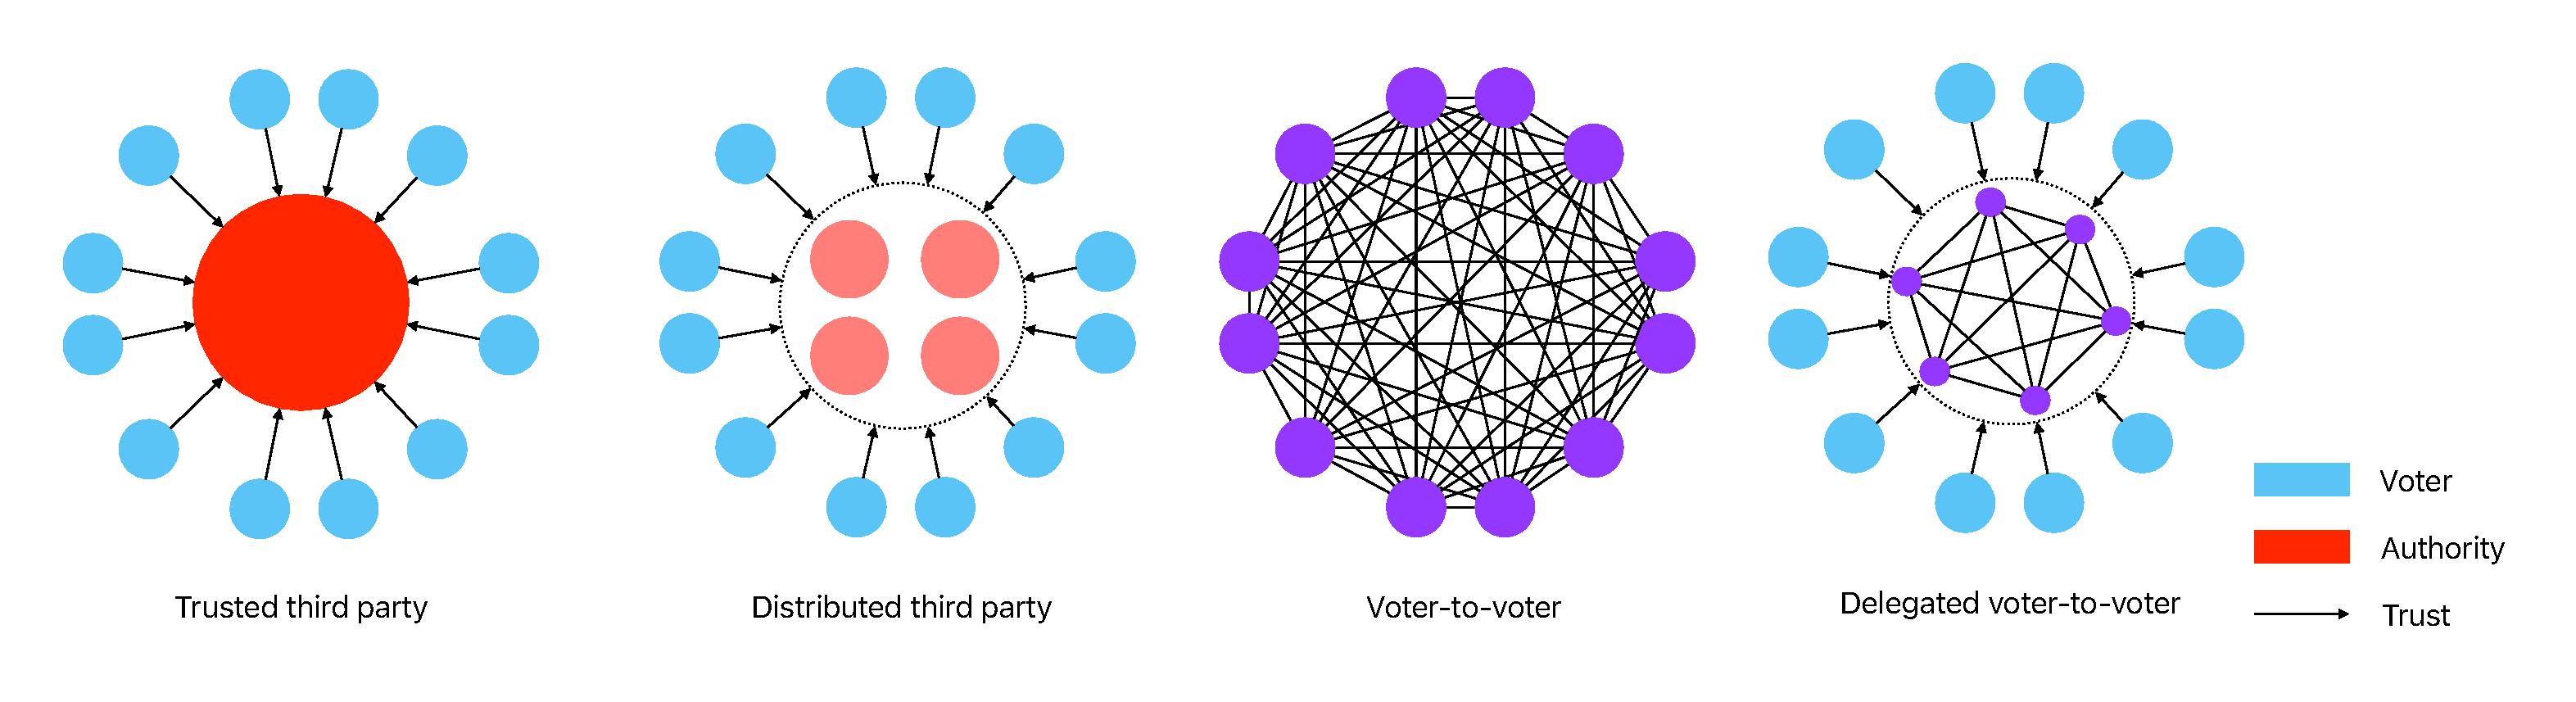
\includegraphics[width=\textwidth]{trust-models-voting.pdf}
    \caption{Four trust models: trusted third party, distributed authorities, peer-to-peer, delegated voter-to-voter}
    \label{fig:trust-models}
\end{figure}

\section{Related work}
Most Internet protocols rely on a trusted third party. They differ in what the server can or cannot do. The honesty of the trusted third party determines either anonymity, privacy or coercion resistance properties.

Most of the current reserach on internet voting protocols uses some kind of blockchain for integral and transparent storage. 
Voatz~\cite{mooreWestVirginiaMobile2019}, 
Polys~\cite{PolysOnlineVoting}, 
OpenVoteNetwork~\cite{haoAnonymousVotingTworound2010}, MACI~\cite{ethereumfoundationMinimalAntiCollusionInfrastructure2022}.

However some projects achieve similar properties without using blockchain. Projects like Civitas, Swisspost/Scytl, iVoting, or ElectionGuard use some kind of distributed authorities to run the voting process. The trust model usually is $N \textrm{ of } N$ where all authorities have to work as expected. All the computation is done using some kind of Multi-Party Computation (MPC) protocol~\cite{boweMultipartyProtocolConstructing2018}.
These systems are not fully decentralised as they are based on a closed set of trusted entities called Guardians. In practice they are "Election Officials, Trustees Canvass Board Members, Government Officials or other trusted authorities who are responsible and accountable for conducting the election"~\cite{ElectionGuardWhoGuardian}.


Solutions built on public blockchains require voters to pay transaction fees.

Solutions built on private blockchains still need to be hosted somewhere, which costs money or creates a high entry point for non-technical people.

Compared to other public-blockchain-based solutions, our solution is free, which is arguably a big deal—paying for a vote must reduce the turnout.

Compared to private-blockchain-based solutions or ElectionGuard-like systems, in our system, there is no need to run the software on any centralised server(s), which is also arguably a big deal, especially in the case of small, informal voting. Someone has to run this server. For larger organisations like universities, it's not a problem as an IT department is responsible for hosting it. But for small organizations, it can be a problem. For example, small informal teams, NGOs, open-source projects, student projects, start-up teams, student communities, boardrooms, housing associations, or even teams like Delendum. Running the software in a SaaS model, brings us back to the question of "who runs the message board and tallying software and can we trust them?" or even "who pays for it?".

In our solution, voters are running the software, so the question of “who runs the message board and tallying software and can we trust them?” changes to “do we trust that the majority (more concretely m-of-n voters) are honest?” Moreover, as the network is private p2p there is no problem of "who pays for it?". And because it's a private blockchain there are no transaction fees.

Below is a comparison table.

\newcommand{\fullmoon}{\tikz\filldraw[fill=black] (0,0) circle (0.5em);}
\newcommand{\newmoon}{\tikz\draw (0,0) circle (0.5em);}
\newcommand{\rightmoon}{\tikz\draw (0,0) circle (0.5em); \filldraw[fill=black] (0,0) arc (90:270:0.5em) -- cycle;}
\newcommand{\leftmoon}{\tikz\draw (0,0) circle (0.5em); \filldraw[fill=black] (0,0) arc (270:90:0.5em) -- cycle;}
\newcommand{\halfmoon}{\tikz\draw (0,0) circle (0.5em); \filldraw[fill=black] (0,-0.5em) rectangle (0,0.5em);}


\begin{table*}[!h]
\centering
\newcommand{\YES}{\cellcolor{red!50}Yes}
\newcommand{\NO}{\cellcolor{green!50}No}
\caption{A comparative analysis of three types of internet voting systems: Public Blockchain-based, Private Infrastructure-based, and Voter-to-Voter Network-based, highlighting their differences in transaction fees, service costs, user-friendliness, and trust dynamics.}
\begin{tabular}{p{0.2\textwidth}p{0.2\textwidth}p{0.19\textwidth}p{0.17\textwidth}p{0.2\textwidth}}
\noalign{\smallskip}\hline\noalign{\smallskip}
\textbf{Property} & \textbf{Centralised server} & \textbf{Private infrastructure} & \textbf{Public blockchain} & \textbf{Voter-to-Voter network} \\
\noalign{\smallskip}\hline\noalign{\smallskip}
Transaction fees & \NO & \NO & \YES & \NO \\
\hline
Service costs\footnote{The cost of service includes all costs related to implementation, maintenance, and fees} & \cellcolor{yellow!50} Medium & \cellcolor{red!50} High & \cellcolor{green!50} No  & \cellcolor{green!50} No \\
\hline
User-Friendliness & \cellcolor{green!50} High & \cellcolor{green!50}High & \cellcolor{red!50} Low & \cellcolor{yellow!50} Medium \\
\hline
Trust to\footnote{Trust is a broad term that refers to different properties of the system, but most of the time it answers the question of who holds the properties of censorship-resistance, privacy, and/or correctness.} & \cellcolor{red!50} Central authority & \cellcolor{yellow!50} Authorities\footnote{Examples of authorities are: "Election Officials, Trustees Canvass Board Members, Government Officials or other trusted authorities who are responsible and accountable for conducting the election", \href{http://www.electionguard.vote/basics/steps/1_Key_Ceremony/}{source}.} & \cellcolor{yellow!50} Miners & \cellcolor{yellow!50} Voters  \\
\noalign{\smallskip}\hline

\hline
\end{tabular}
\end{table*}

\section{System Architecture}
Designig a user application that is intended to work in peer-to-peer model is a complex task. The main challenge is to overcome the networking problems, weak availability and limited resources of end-devices such as smartphones and laptops.

\section{Voting Protocol}
Our voting protocol is a combination of 3-round voting scheme proposed in~\cite{schoenmakersLectureNotesCryptographic2018}, multi-candidate encoding proposed in~\cite{haoAnonymousVotingTworound2010}, and Federated DKG that we propose in this paper. 

We use Threshold ElGamal Cryptosystem which guarantees the decryptiability even in case of unavaiable guardians.

\paragraph*{Assumptions}
\begin{enumerate}
    \item All communication is done over a public Message board.
    \item Authenticated public channels are available for every participant, achieved by a public message board and digital signatures.
    \item Private channels are available for every participant, achieved by a public message board, and ElGamal public key encryption.
    \item The set of all $n$ participants $\vec{P} = \{P_1,\dots,P_n\}$ is publicly known. 
    \item Each participant $P_i$ consists of key pair $(s_i, P_i)$, where $s_{i} \in_{R} \mathbb{Z}_q$ is a randomly selected secret key, and $P_{i} = s_i \times G$ is the corresponding public-key. We use the same notation for a party and its public key, $P_i$, as parties are identified by their public keys only.
    \item We use Elliptic Curve Cryptography, specifically \href{babyJubJub curve}{https://z.cash/technology/jubjub/}.
    \item \begin{enumerate}
        \item Participation in the protocol is equivalent to agreeing to:
        \item Elliptic Curve $E(\mathbb{Z}_q)$, with the base (generator) point on the curve $G$;
        \item set of eligible voters (participants) $\vec{P}$, where $n$ is the number of all voters;
        \item candidate options $\vec{C}=\{C_1, \dots, C_l\}$, where $l$ is the number of all candidates.
    \end{enumerate}
    \item Public-key encryption is realised using ElGamal cryptosystem. $EG_{P}(\cdot)$ is the encryption algorithm for public key $P$, and $EG_{s}(\cdot)$ is the decryption algorithm using corresponding secret key $s$.
    \item Each participant $P_i$ consists of key pair $(sk_i, P_i)$, where $sk_{i} \in_{R} \mathbb{Z}_q$ is a randomly selected secret key and $P_{i} = sk_i \times G$ the corresponding public key. We use the same notation for a party and its public key, $P_i$, as parties are identified by their public keys only.
\end{enumerate}


\subsection{Federated Distributed Key Generation}
The goal of DKG protocol is to jointly generate the voting key-pair without any party learning the secret (decryption) key. Each party $P_1,\dots,P_n$ learns only its share of the secret (decryption) key, while public (encryption) key is publicly known. Moreover we want the threshold property, meaning that, not every party that participated in the key generation needs to participate in the tally phase.

\subsubsection*{Secret Sharing}

Threshold secret sharing can be done using Shamir Secret Sharing (SSS), which allows a dealer to encode secret key $s$ into a random polynomial $f(X) = a_0 + a_1X + a_2X^2 + \dots + a_{t-1}X^{t-1}$, where $a_0,a_1,\dots,a_{t-1} \in_R \mathbb{F}_q$; the secret key $s=a_0=f(0)$ and $t-1$ is the degree of polynomial. Following a Lagrage Theorem, $t$ number of points on the polynomial $f(X)$ allows for reconstructing the polynomial and hence extract secret key by computing $s = a_0 = f(0)$. The shares are distributed to parties $P_i, 1 \leq i \leq n$, by evaluating function at a corresponding point $(x=i,y=f(i))$. The polynomial of degree $t$ can be reconstructed with $t+1$ points using Lagrange Interpolation.

\subsubsection{Distributed Key Generation}
Since we don't want any party to become a dealer (and learn the secret $decryption$ key), we have to distribute the generation of polynomial $\mathbf{f}(X) \in_R \mathbb{Z}_q[X]$ across all parties $\mathbb{P}$. It is done by having each party pick a random polynomial $f_{i}(X) \in \mathbb{Z}_q[X]$, and then define the final polynomial $$\mathbf{f}(X)=\sum_{i=1}^{n}f_i(X)$$. Hence, the voting secret (decryption) key $\mathbf{d}$ and voting public (encryption) key $\mathbf{E}$ are: $$\mathbf{d}=\mathbf{f}(0)$$ $$\mathbf{E}=\mathbf{d}\times G$$. 

To prevent misbehaviour of parties (sending arbitrary values) we use a more sophisticated version of SS called Publicly Verifiable Secret Sharing (\href{PVSS}{https://www.win.tue.nl/~berry/papers/crypto99.pdf}), which involves zero-knowledge proofs attesting that the correct relation between values holds.


\subsubsection{Dynamic Distributed Key Generation}
Distributed Key Generation in its original form requires known and fixed number of participants. It's because, underneath, it relies on SSS which uses polynomials of known degree $t$. The degree is fixed at the beginning of the protocol and can not be changed.

\textbf{We want the DKG phase to be optional}, so the total number of participants is unknown, and so the $t$ is also unknown. As a result, we need a scheme that allows for dynamic updating the number of participants and the threshold.

To our best knowledge, the scheme which allows for dynamic DKG~\cite{delerableeDynamicThresholdPublickey2008} requires all parties to be online for the duration of the DKG (possible a few hours). It's done by reconstructing the key by current participants and resharing it again with the new participant.

We believe it is an unpractical assumption. We want the protocol to be non-interactive, meaning that the party sends only one message and then can leave.

% consider this path of reasoning:
% - We want the DKG and Tally rounds to be optional
% - Threshold Encryption works on Shamir Secret Sharing (SSS)
% - SSS works on polynomials
% - Polynomials have to have a defined fixed degree $t$
% - We want the DKG phase to be optional, so the total number of participants is unknown, and so the $t$ is also unknown
% - Therefore, we can not define the polynomial of unknown size


\subsection{Federated Distributed Key Generation}

We propose a novel technique for dynamic DKG that works similarly to \href{Stellar Consensus Protocol}{https://developers.stellar.org/docs/fundamentals-and-concepts/stellar-consensus-protocol}~\cite{mazieresStellarConsensusProtocol2015}.

Every party can (but does not have to) participate in the DKG phase. The actual number of parties that participate is denoted by $m$ where the maximum number is $n$. Since we focus on small scale votings where participants know each other, we make a social assumption, that each participant trusts $k$ other parties. Then we chose a threshold $t$ of parties, which allows for key reconstruction. Numbers $k$ and $t$ are public parameters agreed by each party.

add figure FDKG.png

\begin{figure}
    \centering
    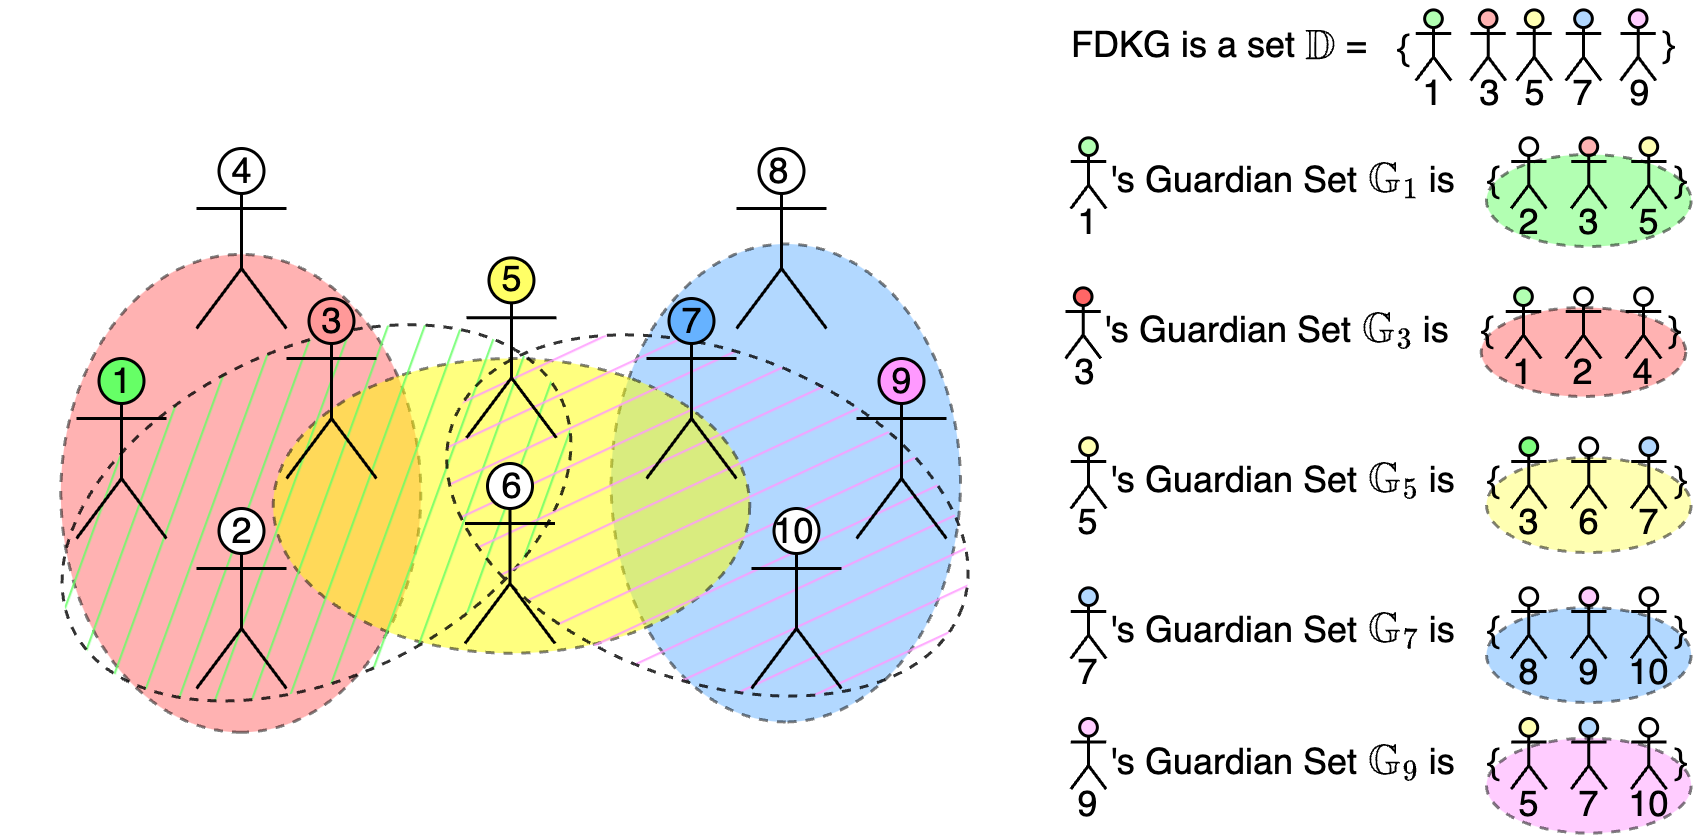
\includegraphics[width=\textwidth]{FDKG.png}
    \caption{Federated Distributed Key Generation}
    \label{fig:FDKG}
\end{figure}

For each party $P_i \in \mathbb{D}$, where $\mathbb{D} \subseteq  \mathbb{P}$ is a subset of parties participating in DKG:
- Chose a guardian set of $k$ parties  $\mathbb{G}_i=\{P_{i_1},P_{i_2},\dots,P_{i_k}\}\subseteq \mathbb{P}/P_i$
- Sample a random polynomial $f_{i}(X) \in_R \mathbb{Z}_q[X]$ of degree $t-1$
- Compute decryption (secret) key $d_{i}= f_i(0)$ and encryption (public) key $E_{i} = d_i \times G$.
- Create a t-of-k access structure for $d_i$ using Publicly Verifiable Secret Sharing (PVSS)
- For each guardian $P_{i,j} \in \mathbb{G}_i$, $1 \leq j \leq k$, create a secret share $f_i(j)$, encrypt it $C_{i,j}=\texttt{Enc}_{P_j}(f_i(j))$ and create a zero-knowledge proof $\pi$ = “I know $f_i$ s.t. given $j, P_j$, and $C_{i,j}$, the $C_{i,j}$ is an encrypted value of a polynomial $f_i(\cdot)$ applied to $j$“
- Broadcast $(E_i,C_{i,j}, \pi)$


\subsubsection{Private Channel}

\begin{algorithm}
    \SetAlgoNlRelativeSize{0}
    \SetAlgoNlRelativeSize{-1}
    \SetAlgoNlRelativeSize{1}
    \SetKwInOut{Input}{Input}
    \SetKwInOut{Output}{Output}
    \caption{Encryption\_P}
    
    \Input{A scalar $s$}
    \Output{A tuple $(C1, C2, \Delta)$}
    
    $k \gets_\$ \mathbb{Z}$\;
    $r \gets_\$ \mathbb{Z}$\;
    $C1 = k \cdot G$\;
    $M = G \cdot r$\;
    $C2 = P \cdot k + M$\;
    $\Delta = s - M.x$\;
    \Return $(C1, C2, \Delta)$\;
\end{algorithm}

\begin{algorithm}
    \SetAlgoNlRelativeSize{0}
    \SetAlgoNlRelativeSize{-1}
    \SetAlgoNlRelativeSize{1}
    \SetKwInOut{Input}{Input}
    \SetKwInOut{Output}{Output}
    \caption{Decryption\textsubscript{sk}}
    
    \Input{A tuple $(C_1, C_2, \Delta)$}
    \Output{A scalar $s$}
    
    $M = C_2 - sk \cdot C_1$\;
    $s = M.x - \Delta$\;
    \Return $s$\;
\end{algorithm}

\paragraph*{State after round 1. FDKG}

After the DKG has been completed (once it reached $n$ messages or after some predefined period). The message board state looks as follows:
- $\{E_{i} : 1 \leq i \leq m\}$, shares of voting public key.
- $\{\sigma_{i} : 1 \leq i \leq m\}$, proofs of exponents.
- $\{\{EG_{P_{j}}(\vec{d}_{i}[j]) : j \in \{1\dots k\}\} : 1 \leq i \leq m \}$, encrypted shares of shares of voting secret key.

The voting encryption key $\textbf{E}$ can be reconstructed by everyone by computing $\mathbf{E}=\sum_{i=1}^{n} E_{i}$.

The share of voting decryption key $\mathbf{D_i}$ can be reconstructed by party $P_i$ by computing $\mathbf{D}_{i}=\sum_{j=1}^{m} EG_{s_{i}}(d_{ji})$.


\subsection{Casting votes}

Every party can (but does not have to) participate in the voting phase. The actual number of parties that participated is denoted by $k$ where the maximum number is $n$.

For each voter $P_i \in \mathbb{V}$, where $\mathbb{V} \subseteq  \mathbb{P}$ is a subset of parties participating in voting:

\begin{enumerate}
    \item Select a vote $v_{ij} \in \{0,1\} \simeq \{\textrm{"no", "yes"}\}$ for each candidate $j \in \{1 \dots l\}$.
    \item Compute a ballot using ElGamal encryption for $B_i = (r_i G,\ r_i \mathbf{E} + v_{i1} H_1 + \dots + v_{il} H_l)$, where 
    \item \begin{enumerate}
        \item $r_{i} \in_{R} \mathbb{Z}_q$ is a blinding factor for user $i$, and 
        \item $H_{1,}\dots, H_{l}$ are independent generators (one for each candidate).
    \end{enumerate}
    \item Compute a zero-knowledge proof $\pi$ = “I know $r_i, v_{i1},\dots,v_{ij}$ s.t.$\sum_{j= 1 \dots l}v_{ij}=1$ and $\forall_{j=1}^{l}v_{ij}=1 \lor v_{ij}=0$ and $B_i$ is a correctly encrypted ballot using those values”
    \item Broadcast $(B_i,\pi)$.
\end{enumerate}

\paragraph{State after voting}

After the voting phase has completed (once it reached $n$ messages or after a predefined period). The message board state is appended by:
- $\{(B_{i}, \sigma_i) : 1 \leq i \leq k\}$, set of encrypted votes casted by $k$ voters, along with ZKPs showing that $v_{ij}$ is one of $\{0,1\}$.

\subsection{Tally}

Tally consists of two phases
\subsubsection{Online Tally}

For each party $P_i \in \mathbb{T}$, where $\mathbb{T} \subseteq  \mathbb{D}$ is a subset of parties participating in the Threshold ElGamal Decryption. $\mathbb{T}$ must include at least $t \leq k$ parties from every set of guardians $\mathbb{G}_1,\dots,\mathbb{G}_{|\mathbb{D}|}$.
\begin{enumerate}
    \item Sum the first part of the ballots $A = \sum_{i \in 1 \dots |\mathbb{V}|} C1_i = \sum_{i \in 1 \dots |\mathbb{V}|} r_{i} \times G$, where $(C1_i,C2_i)=B_i$.
    \item  Calculate the share of the decryption key $d_i=\sum_{f_j(i) \in S_i} f_j(i) \lambda_{j,i}$, where $S_i$ is a set of shares $f_j(i)$, where $P_i$ is in $P_j$'s guardian set $\mathbb{G}_j$, and $\lambda_{j,i}=\prod_{k \in \mathbb{G}_j \setminus \{i\}} \frac{k}{k-i}$ denotes Lagrange coefficients. 
    \item Calculate partial decryption $A_i = A \cdot d_i$.
    \item Compute a zero-knowledge proof $\pi$ = “I know all shares $f_j(i)$ from encrypted shares $C_{j,i}=\texttt{Enc}_{P_i}(f_j(i))$ s.t. $A_i = A \cdot d_i$"
    \item Broadcast partial decryption $(A_i, \pi)$
\end{enumerate}

\subsubsection{Offline Tally}

Anyone can calculate the voting results:
\begin{enumerate}
    \item Sum the first part of the ballots $C2 = \sum_{i \in 1 \dots |\mathbb{V}|} C2_i = \sum_{i \in 1 \dots |\mathbb{V}|} r_i \mathbf{E} + v_{i1} H_1 + \dots + v_{il} H_l$, where $(C1_i,C2_i)=B_i$
    \item Sum the partial descriptions $Z=\sum_{i \in 1 \dots |\mathbb{V}|} A_i = \sum_{i \in 1 \dots |\mathbb{V}|} A \sum_{f_j(i) \in S_i} f_j(i) \lambda_{j,i} = A \cdot d$
    \item The decryption is $M=C2-Z=x_1 H_1 + \dots + x_l H_l$
    \item $M=C2-Z=x_1 H_1 + \dots + x_l H_l$ because,
    \item $\begin{aligned} M&=C2-Z \\
        &= \sum_{i=1}^k ( r_{i} \times \mathbf{E}) + H_1 \times \sum_{i=1}^k v_{i1} + \dots + H_l \times \sum_{i=1}^k v_{il} - Z\\
        &= \sum_{i=1}^k ( r_{i} \times \mathbf{E}) + H_1 \times \sum_{i=1}^k v_{i1} + \dots + H_l \times \sum_{i=1}^k v_{il} - \sum_{i=1}^k r_{i} \times \mathbf{E}\\
        &= H_1 \times \sum_{i=1}^k v_{i1} + \dots + H_l \times \sum_{i=1}^k v_{il}\\
        &= x_1 H_1 + \dots + x_l H_l\\
        \end{aligned}$
    \item To extract $x_c$ we have to solve Elliptic-Curve Discrete Logarithm Problem. However, because $x_c$ is a small number $0 \leq x_c \leq |\mathbb{V}|$ it is feasible. To extract each $x_i$ we use the technique described in~\cite{haoAnonymousVotingTworound2010}.
\end{enumerate}

\section{zkSNARKs for Protocol Adherence}

\section{Privacy and Availability Considerations}

\section{System Implementation}

\subsection{Consensus and Networking}

\begin{figure}
    \centering
    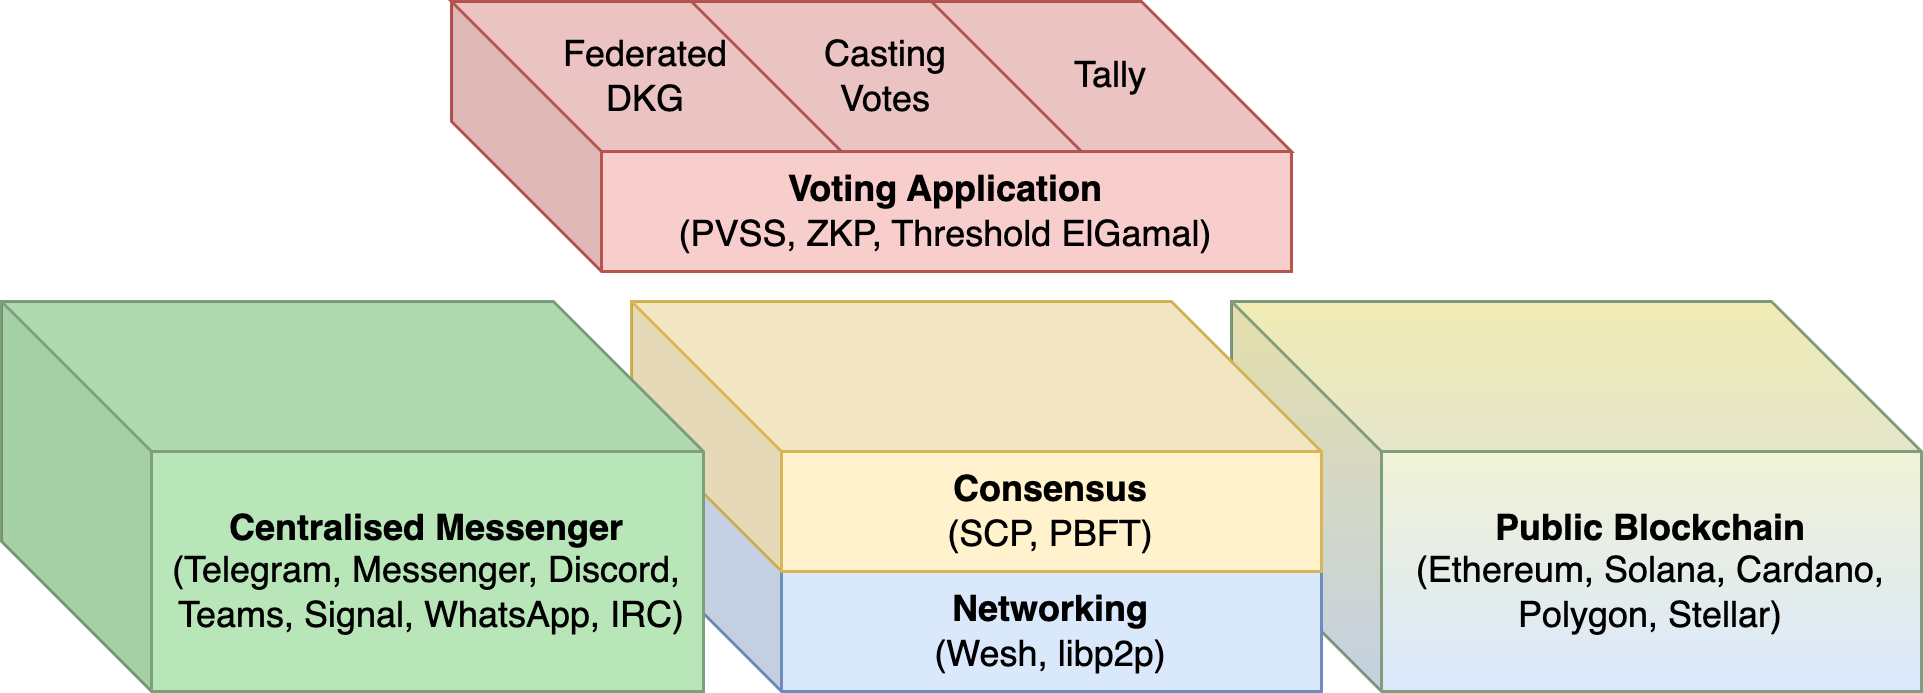
\includegraphics[width=\textwidth]{stack-bc.png}
    \caption{Federated Distributed Key Generation}
    \label{fig:FDKG}
\end{figure}

- Ad-hoc blockchain network
- p2p networking via async mesh network https://wesh.network/
- FBA or Tendermint
- Or, a public blockchain with ERC4337 paymaster to cover the transaction costs

\section{Experimental Results}

\begin{table}
\centering
\caption{Execution time of the PLONK prover in seconds.}
\begin{tabular}{|c|c|c|c|c|}
    \hline
    \multicolumn{5}{|c|}{PLONK} \\
    \hline
    \multicolumn{3}{|c|}{PVSS} & \multirow{2}{*}{Encrypt ballot} & \multirow{2}{*}{Partial decryption} \\
    \cline{1-3}
    1 of 2 & 2 of 3 & 3 of 4 & & \\
    \hline
    232.972 & 249.835 & 622.324 & 59.709 & 27.363\\
    \hline
\end{tabular}
\end{table}

\begin{table}
\centering
\caption{Execution time of the Groth16 prover in seconds.}
\begin{tabular}{|c|c|c|c|c|}
    \hline
    \multicolumn{5}{|c|}{Groth16} \\
    \hline
    \multicolumn{3}{|c|}{PVSS} & \multirow{2}{*}{Encrypt ballot} & \multirow{2}{*}{Partial decryption} \\
    \cline{1-3}
    1 of 2 & 2 of 3 & 3 of 4 & & \\
    \hline
    3.026 & 5.002 & 5.274 & 1.583 & 1.089\\
    \hline
\end{tabular}
\end{table}

%TODO: 
\section{Discussion}

\section{Conclusion and Future Work}

\section{Acknowledgments}


\bibliographystyle{IEEEtran}
\bibliography{bibliography}

\end{document}